\chapter{Chi-square Distribution ($X \sim \chi^2_k$) \cite{ism-1,wiki/Chi-squared_distribution}} \label{Chi-square Distribution}

\begin{table}[H]
    \begin{minipage}{0.49\linewidth}
        \begin{figure}[H]
            \centering
            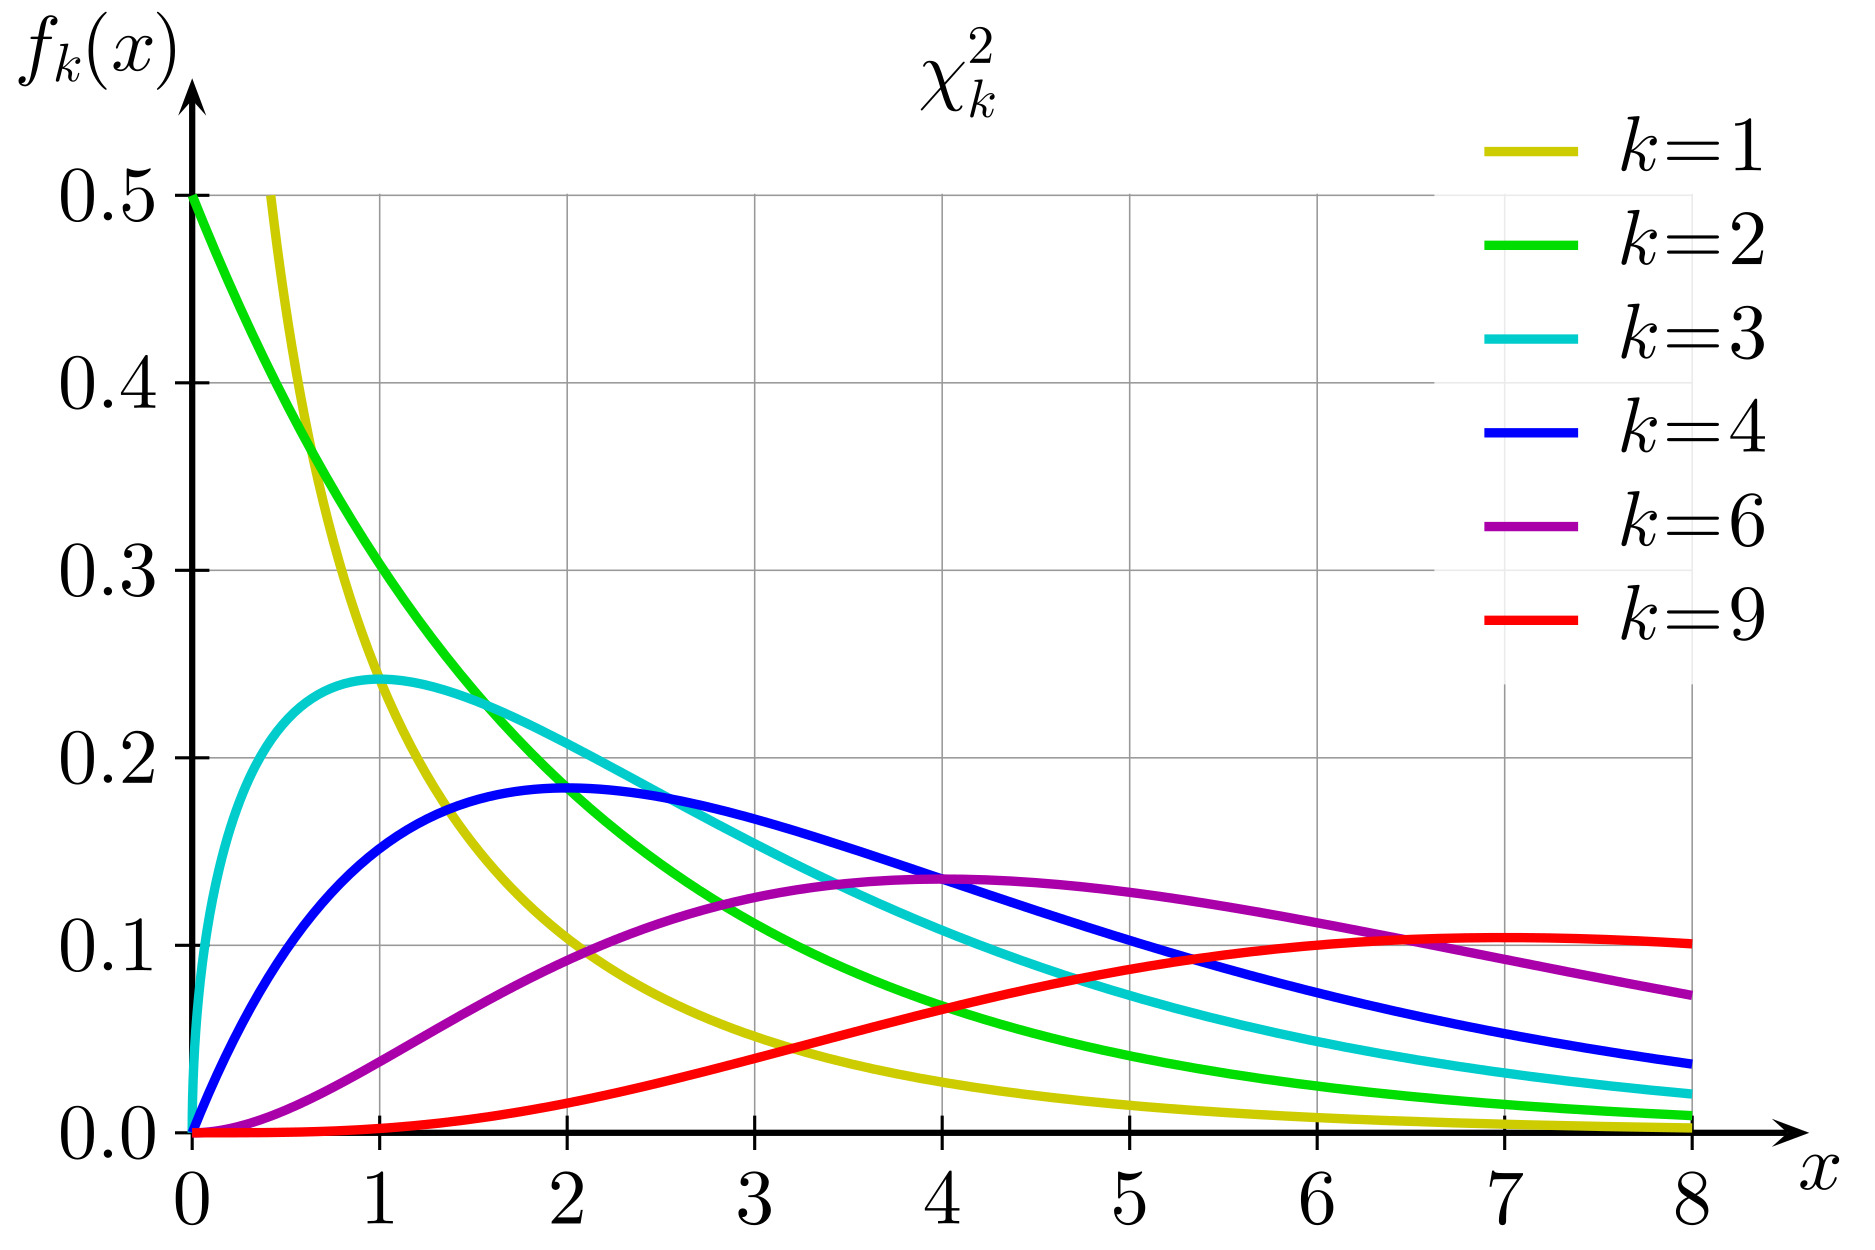
\includegraphics[width=\linewidth, height=4cm, keepaspectratio]{Pictures/distributions/Chi-square_pdf.jpg}
            \caption{Chi-square Distribution: PDF}
        \end{figure}
    \end{minipage}
    \hfill
    \begin{minipage}{0.49\linewidth}
        \begin{figure}[H]
            \centering
            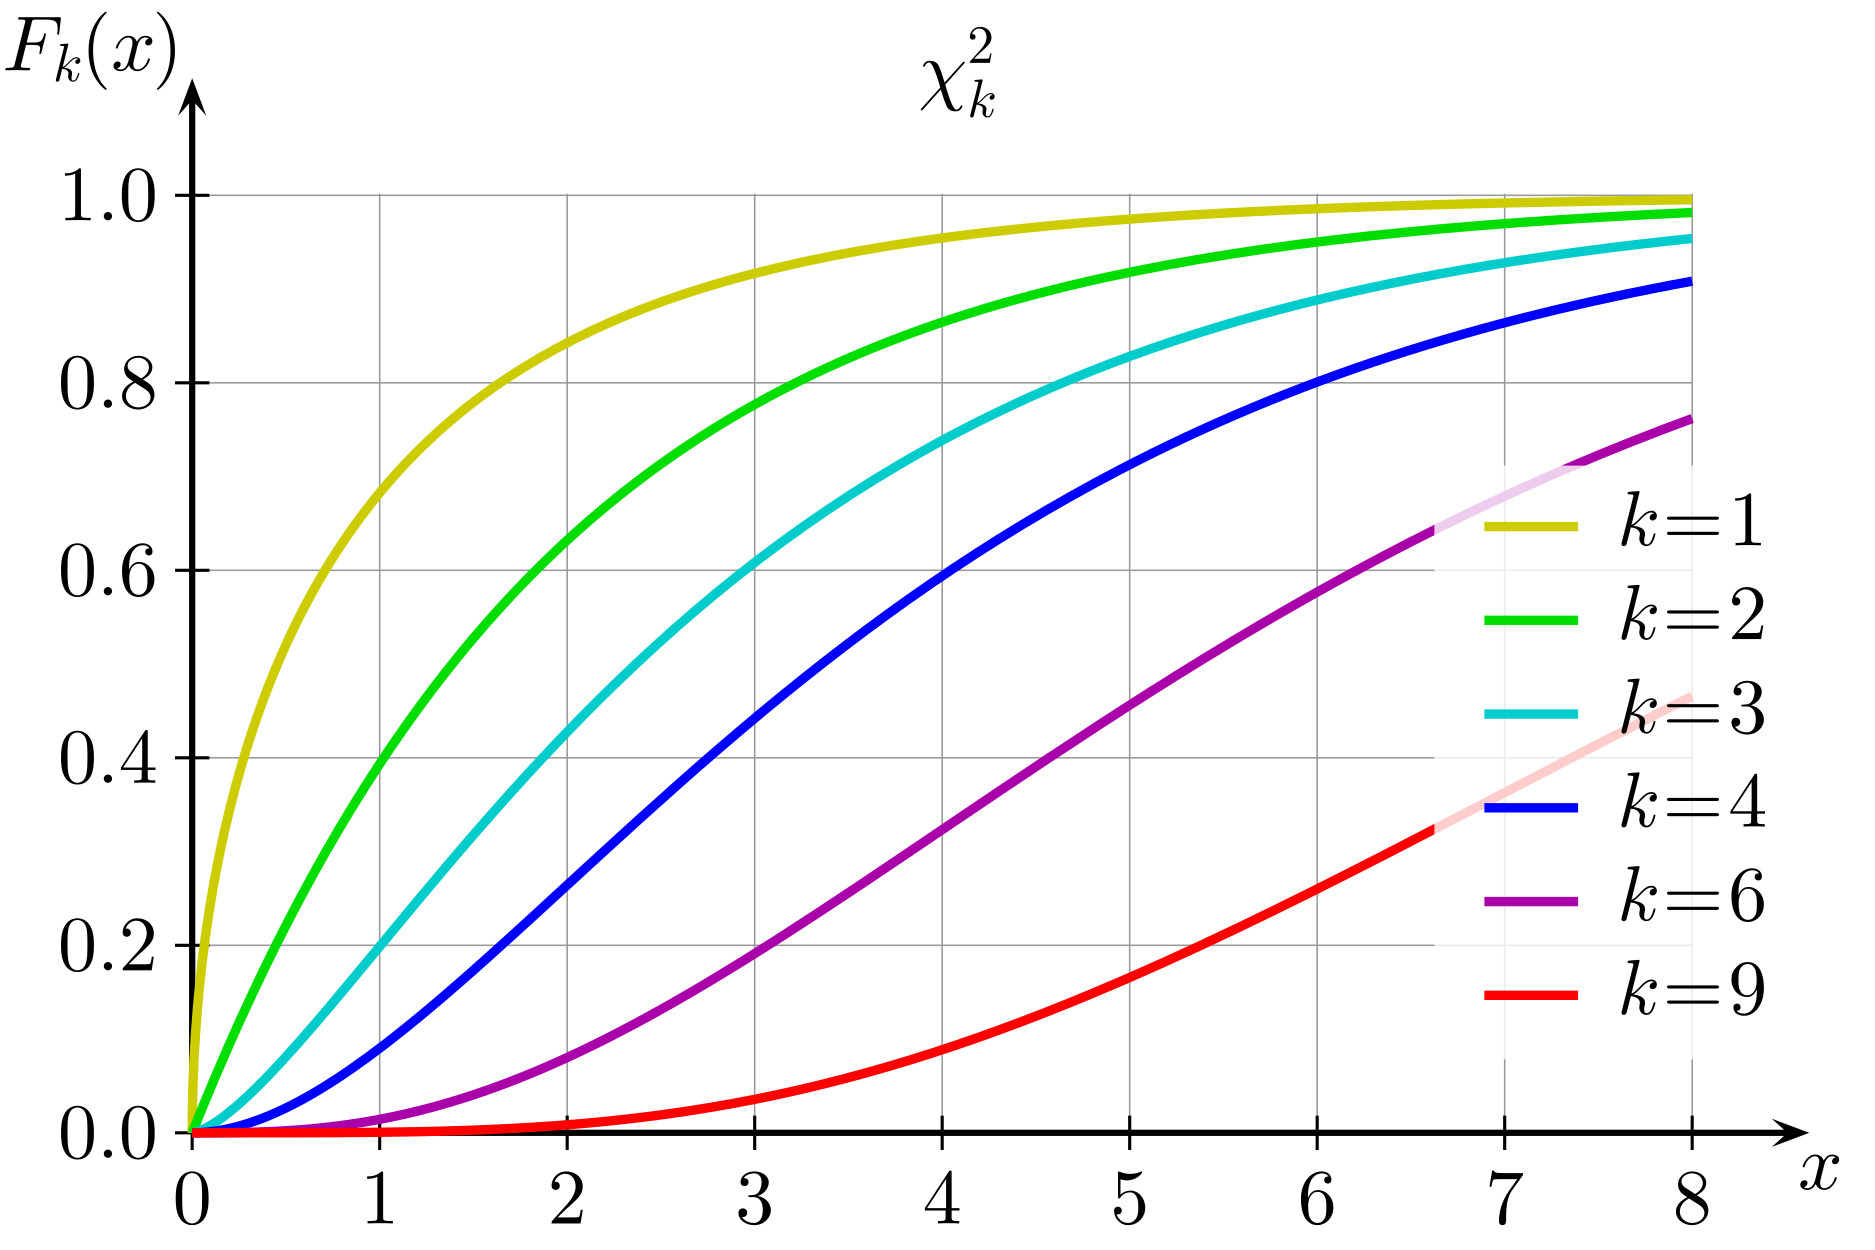
\includegraphics[width=\linewidth, height=4cm, keepaspectratio]{Pictures/distributions/Chi-square_cdf.jpg}
            \caption{Chi-square Distribution: CDF}
        \end{figure}
    \end{minipage}
\end{table}

\renewcommand{\arraystretch}{2}
\begin{longtable}{|m{6cm}|p{9cm}|}
    \hline
    \multicolumn{2}{|c|}{\textbf{Chi-square Distribution - Info} \cite{wiki/Chi-squared_distribution}} \\
    \hline\endfirsthead

    \hline
    \multicolumn{2}{|c|}{\textbf{Chi-square Distribution - Info - contd.} \cite{wiki/Chi-squared_distribution}} \\
    \hline\endhead
    
    \hline\endfoot
    \hline\endlastfoot

    \textbf{Notation} &
    ${\displaystyle \chi ^{2}(k)\;}$ or ${\displaystyle \chi _{k}^{2}\!}$
    \\ \hline

    \textbf{Statistical parameters} & 
    ${\displaystyle k\in \mathbb {N} ^{*}~~}$ (known as "degrees of freedom")
    \\ \hline
    
    \textbf{Support} &
    ${\displaystyle x\in [0,+\infty )\;}$
    \\ \hline

    \textbf{Probability Density Function (PDF)} & 
    ${\displaystyle {\dfrac {1}{2^{k/2}\Gamma (k/2)}}\;x^{k/2-1}e^{-x/2}\;}$
    \\[1ex] \hline
    
    \textbf{Cumulative distribution function (CDF)} & 
    ${\displaystyle {\dfrac {1}{\Gamma (k/2)}}\;\gamma \left({\dfrac {k}{2}},\,{\dfrac {x}{2}}\right)\;}$
    \\ \hline

    \textbf{Mean} & 
    $k$
    \\[1ex] \hline

    \textbf{Median} & 
    ${\displaystyle \approx k{\bigg (}1-{\dfrac {2}{9k}}{\bigg )}^{3}\;}$
    \\[1ex] \hline

    \textbf{Mode} & 
    ${\displaystyle \max(k-2,0)\;}$
    \\ \hline

    \textbf{Variance} &
    $2k$
    \\[1ex] \hline

    \textbf{Skewness} &
    ${\displaystyle {\sqrt {\dfrac{8}{k}}}\,}$
    \\[1ex] \hline

    \textbf{Excess kurtosis} &
    ${\displaystyle {\dfrac {12}{k}}}$
    \\[1ex] \hline

    \textbf{Entropy} &
    ${\displaystyle {{\dfrac {k}{2}} +\log \left(2\Gamma {\Bigl (}{\dfrac {k}{2}}{\Bigr )}\right)+\left(1-{\dfrac {k}{2}}\right)\psi \left({\dfrac {k}{2}}\right)}}$
    \\[1ex] \hline

    \textbf{Moment-generating function (MGF)} &
    ${\displaystyle (1-2t)^{-k/2}{\text{ for }}t<{\frac {1}{2}}\;}$
    \\[1ex] \hline

    \textbf{Characteristic function (CF)} &
    ${\displaystyle (1-2it)^{-k/2}}$
    \\[1ex] \hline

    \textbf{Probability-generating function (PGF)} &
    ${\displaystyle (1-2\ln t)^{-k/2}{\text{ for }}0<t<{\sqrt {e}}\;}$
    \\[1ex] \hline

\end{longtable}
\renewcommand{\arraystretch}{1}

\begin{enumerate}[itemsep=0.2cm]
    \item Confidence Interval:
    \begin{enumerate}[itemsep=0.2cm]
        \item $V_{n-1}^2 = (n-1)S^2/\sigma^2 \sim \chi_{n-1}^2$

        \item $p$th quantile of the chi-square distribution with $n - 1$ DOF: $x_p(f_{\chi^2})$

        \item $
            \hfill
            Pr(V_{n-1}^2 \leq x_p(f_{\chi^2})) = p
            \hfill
            Pr(V_{n-1}^2 > x_{1-p}(f_{\chi^2})) = p
            \hfill
        $

        \item $
            Pr(\sigma^2 < (n-1)S^2/x_{1-p}(f_{\chi^2})) = p 
        $

        \item $1 - 2p$ confidence interval for the variance $\sigma^2$ is:
        \[[
            (n-1)S^2/x_{1-p}(f_{\chi^2}), 
            \hspace{0.2cm}
            (n-1)S^2/x_{p}(f_{\chi^2})
        )\]

    \end{enumerate}

\end{enumerate}
































